% Copyright (c) 2014,2016,2018 Casper Ti. Vector
% Public domain.

\chapter{云环境中的异构硬件为人工智能带来的机遇与挑战}
% \pkuthssffaq % 中文测试文字。
随着硬件技术的不断发展,云环境中支持机器学习任务的硬件也从单一的CPU变成了包含CPU、GPU、FPGA、TPU以及SGX等安全硬件的异构资源。利用这些异构资源,可以给机器学习任务带来一定增益。例如GPU,TPU和FPGA等硬件的SIMD计算模式天然适合ML这种迭代式、大批量的负载,从而可以大大加速ML训练。而诸如SGX等硬件由让机器学习安全有了从硬件层面得到解决的可能性。

而异构硬件为ML任务带来机遇的同时,也带来了一定的挑战。例如,在公有云共享资源池的背景下,如GPU和FPGA等新兴加速硬件没有成熟和系统的虚拟化方案,用户的使用这些硬件的模式仍然以独占为主。即便是共享,也没有成熟的隔离机制保证性能以及用户之间不会相互干扰。再比如,SGX加持的安全计算环境中,可信内存的大小十分有限,如何在有限的资源下支持可信的模型部署甚至模型训练,是亟待解决的问题。

本章将以加速型硬件GPU和安全型硬件SGX为主,介绍云环境中异构硬件为机器学习任务带来的机遇与挑战。

\section{云环境中机器学习作业对GPU的利用}

本节将先对GPU的现状做简要介绍,包括现代GPU的架构以及常见的GPU API和编程模型。然而,本章将从两个角度展开当前学术界针对ML任务对GPU的利用的研究:1)One Job on Multi GPUs。即一个ML任务需要多个GPU设备。这种情况一般出现在大型模型的分布式训练中。在一个大规模GPU集群中,不同的训练任务对GPU数量的需要可能不一样,如何对这些任务进行调度,使系统的资源利用率最高,同时保证训练任务的性能,是学术界研究的重点问题;2)Multi Jobs on one GPU。即在同一个GPU设备运行多个ML任务。这种情况在资源短缺或多租户的场景下较为常见。

\subsection{GPU简介}

\subsubsection{GPU架构}
GPU,即Graphics Processing Unit,采用了与传统的多核处理器完全不同的架构。GPU的设计围绕和让吞吐率最大化这一原则,提供了上千个简单的计算核心和高带宽内存。这样的实际使得GPU能够使一个应用程序拥有很高的并行度,从而使程序的吞吐率最大化。理想情况下,对于一个GPU应用程序,其包含的若干线程应该分别对应其数据空间的不同位置,而彼此之间由没有因果关联,从而可以并发地执行。与之相反,传统的处理器是为了能更快地执行线性的代码段而优化的。因此其单个核心的复杂度非常高,且单个处理器中的核心数量相对较少。且传统的处理器一般会使用复杂的控制逻辑和较大的本地缓存以处理传统程序中常见的条件分支、上下文切换以及较差的数据本地行。

\begin{figure}[h]
    \centerline{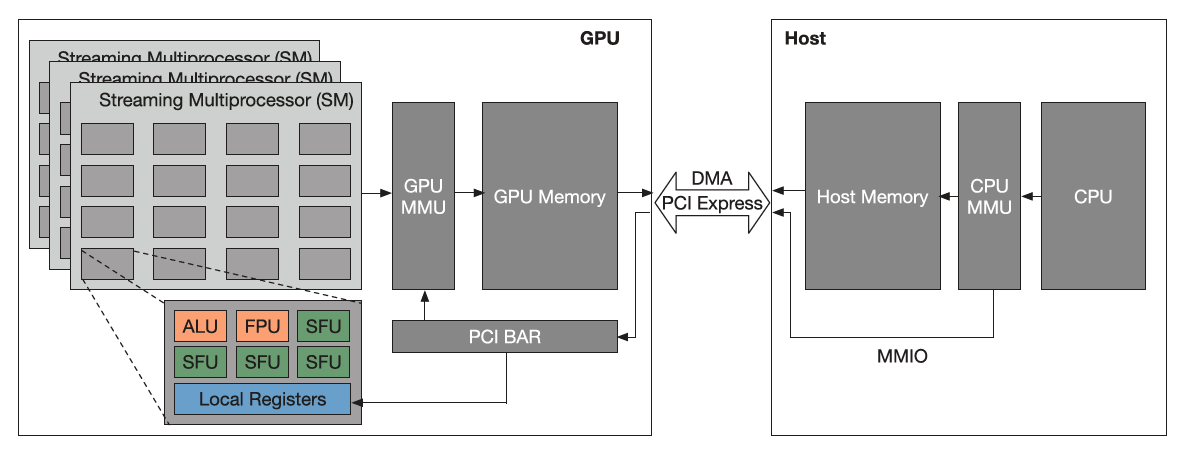
\includegraphics[width=\textwidth]{figures/gpu-arch.png}}
    \caption{GPU系统架构。}
    \label{gpu_arch}
\end{figure}

图~\ref{gpu_arch}展示了一个典型的GPU系统的架构。图中的GPU部分是根据Fermi架构的Nvidia GPU,但是现代的GPU(例如新一代的Nvida GPU和AMD GPU)也遵循类似的设计。一个GPU拥有多个流式处理器(streaming multiprocessor,SM),每一个SM拥有32个计算核心。每个SM也拥有L1数据缓存和低延迟共享内存。每个计算核心拥有本地的寄存器、一个整型计算单元(Integer Arithmetic Logic Unit,ALU)、一个浮点计算单元(Floating Point Unit,FPU)以及若干特殊函数单元(Special Function Units,SFU,用来计算特定的函数值,例如正弦函数sine和余弦函数cosine)。GPU的内存管理单元(MMU)为GPU程序提供虚拟地址空间。MMU会根据应用程序的页表,会将一个GPU地址解析为物理地址。

Host通过PCI高速通道(PCIe)与GPU连接。Host上的CPU通过内存输入/输出映射(MMIO)与GPU进行交互。GPU寄存器以及设备内存可以被CPU通过MMIO接口直接获取。此外,量比较大的数据交换可以通过DMA(Direct Memory Access)实现。DMA可以将数据在设备内存和主机内存之间快速传输。

\subsubsection{GPU API和编程模型}
常用的GPU API和编程模型包括OpenGL,Direct3D,CUDA和OpenCL等,在游戏开发、图像处理、高性能计算等场景下非常常用。

OpenGL是一个利用GPU硬件加速图形处理的库,通常应用于电子游戏、图像处理以及科学计算中的数据可视化。OpenGL实现了一个硬件无关的API,兼容适配不同的底层硬件。

Direct3D是由Microsoft Windows提供的图形库,通常在一些性能敏感的场景中(例如电子游戏)负责图形渲染工作。Direct3D同样实现了硬件无关的API,并且向用户暴露了能够使用GPU高级特性的API,例如Z-buffering,W-buffering等。

CUDA是由Nvidia提供了专为Nvidia GPU适配的并行加速库。CUDA允许开发者在GPU上利用高并行的特点开发特定的程序,这种情形下的GPU被称为GPGPU(General Purpose GPU)。CUDA API是与编程语言高度绑定的,例如C和C++。当前流行的机器学习框架,例如Tensorflow和Pytorch,在存在GPU设备的环境中,都支持利用CUDA对其模型训练进行加速。

OpenCL也是一个并行加速库,其基础功能和CUDA类似,最大的区别在于OpenCL可以被应用于非Nvidia的GPU。

\subsection{One Job on Multi GPUs: 机器学习集群中的GPU调度算法}
%SC 17 Topology-aware
%NSDI 19 Tiresias
%OSDI 20 HiveD
随着深度学习的兴起和快速发展,在计算机视觉、自然语言处理等领域使用的模型参数越来越多,规模越来越大。而对于大规模的深度学习模型,分布式训练+GPU硬件加持几乎成为了标配。分布式训练的场景中,GPU之间的数据传输时有发生。然而在一个多GPU的集群环境中,位于整个系统拓扑结构不同位置的GPU之间的数据传输速度是有很大差异的。

\begin{figure}[h]
    \centerline{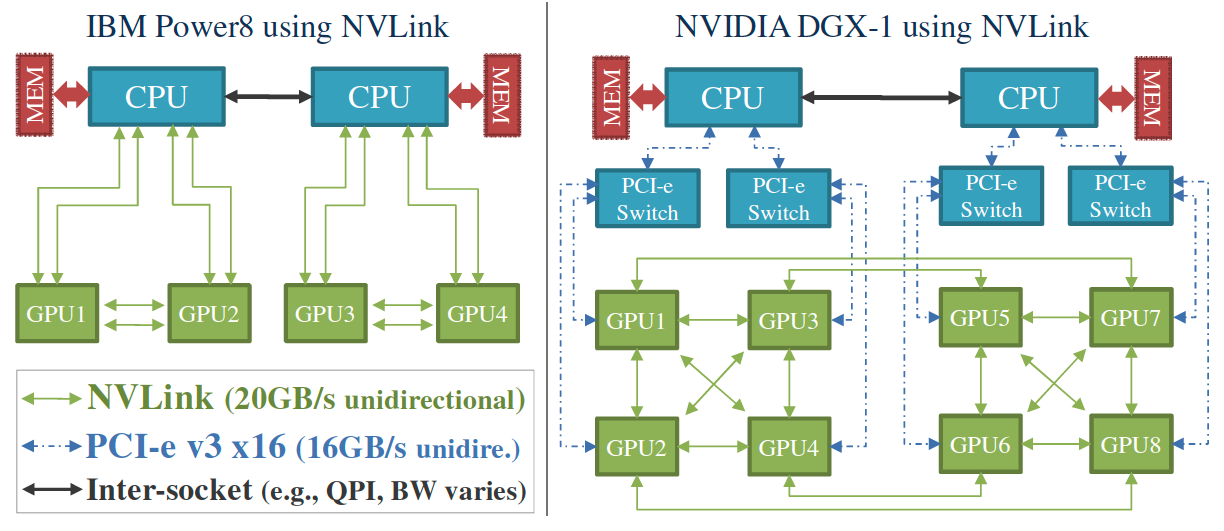
\includegraphics[width=\textwidth]{figures/gpu-topology.png}}
    \caption{GPU拓扑结构示例。}
    \label{gpu_topology}
\end{figure}

图~\ref{gpu_topology}展示了两个GPU服务器中GPU的和其它硬件之间的拓扑结构图。左图为IBM的Power8服务器,有两个CPU和四个GPU。右图嵬NVIDIA和DGX-1服务器,有两个CPU、四个PCI-e桥接器和8个GPU。绿色的线、蓝色的线和黑色的线分别代表NVLink、PCI-e和Intel的QPI三种连接方式,数据传输速度由快到慢。位于同一个CPU socket下的两个GPU(例如左图中GPU1和GPU2)之间的数据传输可以通过NVLink进行,是最快的。位于不同CPU上的GPU,只能通过PCI-e通道和QPI通道进行通信(例如左图中的GPU1和GPU3、右图中的GPU1和CPU)。而如果位于两台不同服务器上的GPU之间需要通信,则除了需要经过上述数据通路之外,还要经过网络传输,即时是万兆网(10Gbps),也要比上述传输方式慢约一个数量级。

\begin{figure}[h]
    \centerline{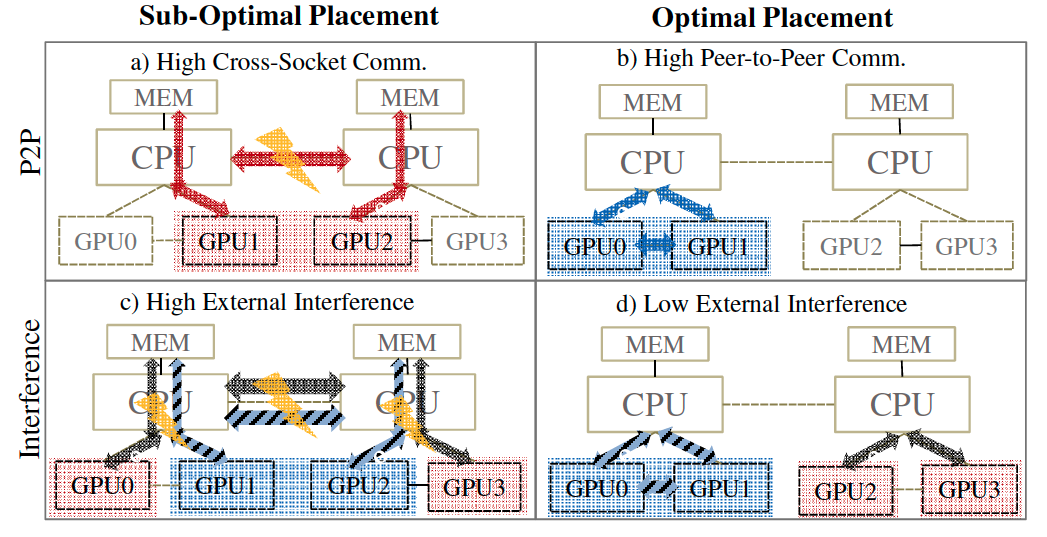
\includegraphics[width=\textwidth]{figures/gpu-top-sub-opt.png}}
    \caption{GPU调度示例。}
    \label{gpu_top_sub_opt}
\end{figure}

因此,在GPU集群中调度分布式ML训练任务时,需要充分考虑GPU之间的拓扑结构,否则可能会造成严重的性能损失。图~\ref{gpu_top_sub_opt}展示了GPU调度的两个例子和与其对应的四种调度方案。上面的两张图对应了P2P(即两个GPU之间需要互相通信)的场景中的两种调度方案,显然右边的方案是更优的方案,因为分配到的两个GPU位于同一个CPU socket上,于左边相比其数据通路具有更高的传输速率。下面的两张图对应了不当分配可能造成的性能干扰。显然,右边的分配方式也是更优的方式,因为左边的分配方式造成了两个Job在数据传输时共用同一条数据通路从而造成竞争,使性能降低。

M. Amaral等人\parencite{amaral2017topology}在2017年提出了一种云环境下基于GPU拓扑结构的调度方法。其将ML任务和集群都抽象成图的形式。在ML的任务图中,图的节点为GPU,节点之间的边代表两个GPU之间存在数据交流。任务图中的边没有权重。在集群的图中,图的节点为CPU,GPU,PCI-e桥接器,CPU socket或者网络交换机。不同节点之间的连线代表这两个节点之间可以相互通信,连线的权重代表通信速度,数值与越小通信速度越快。图~\ref{gpu_graph}表示了图~\ref{gpu_topology}所对应的拓扑结构图。

\begin{figure}[h]
    \centerline{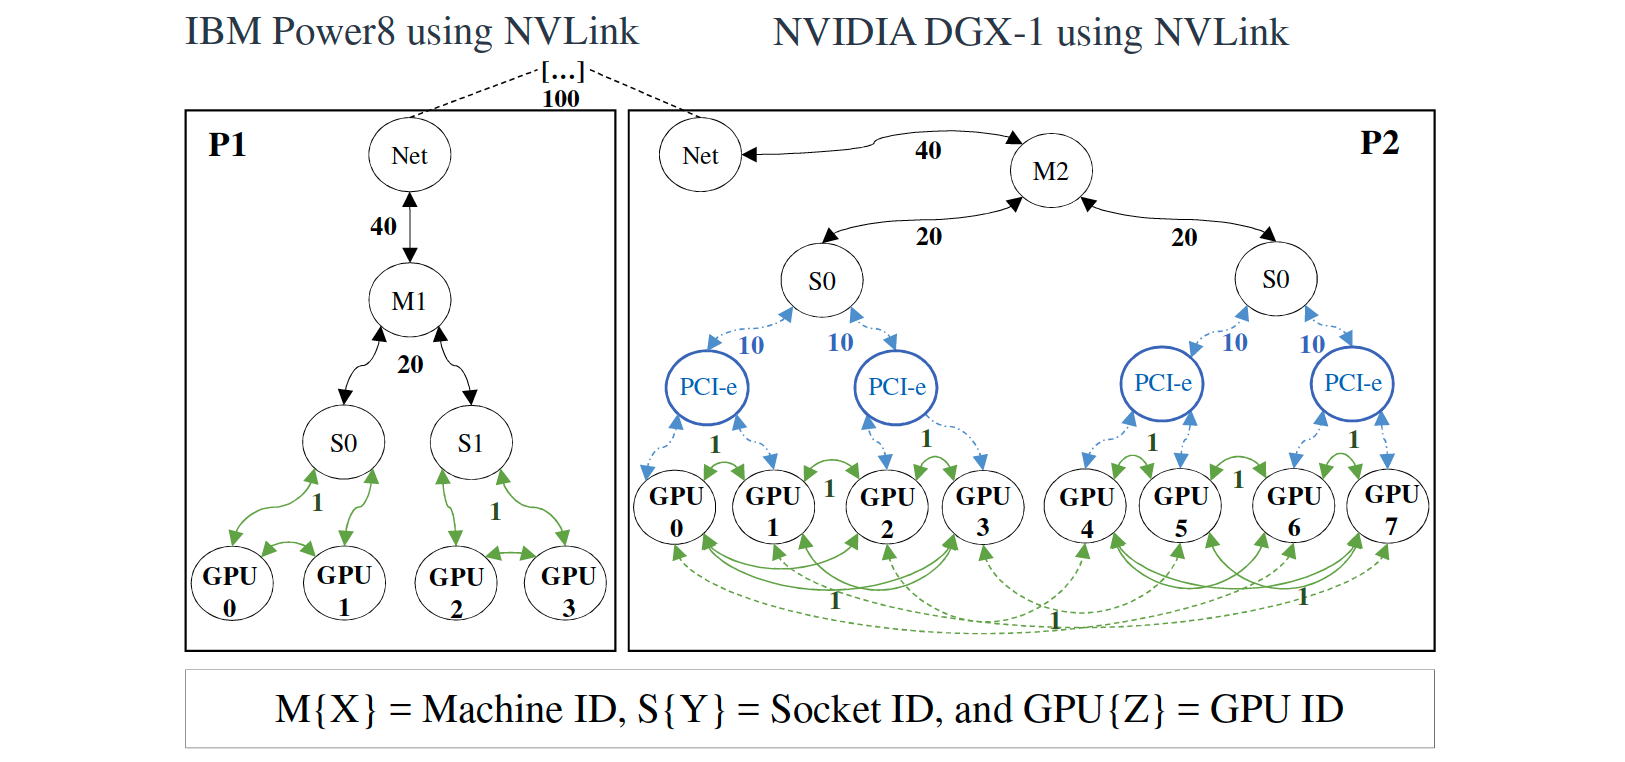
\includegraphics[width=\textwidth]{figures/gpu-graph.png}}
    \caption{GPU拓扑结构图。}
    \label{gpu_graph}
\end{figure}

M. Amaral等人通过对两个图进行匹配并最小化公式~\ref{eq_top_min}中的目标来实现GPU的调度,其中$\alpha^{cc}+\alpha^b+\alpha^d=1$,$t$、$I$和$\omega$分别代表GPU之间的通信代价、来自外部的资源干扰和资源碎片化程度,分子代表实际的值,分母代表最坏情况下的值。该公式旨在综合考虑减小GPU之间的通信代价、降低不同任务之间的干扰以及使整个系统的碎片化尽可能降低,使整个集群处于一个相对最佳的状态。

\begin{equation}\label{eq_top_min}
    MIN\ \alpha^{cc}\frac{t^{cc}}{t_w}+\alpha^b\frac{I^b}{I_w}+\alpha^d\frac{\omega^d}{\omega^w}
\end{equation}

\subsection{Multi Jobs on one GPU: 机器学习集群中的GPU共享机制}
%OSDI 18 Gandiva
%Eurosys 18 Optimus
%ASPLOS 20 SwapAdviosr
%MLSys 20 Salus
\section{云环境中机器学习作业对SGX的利用}

\subsection{SGX技术发展历程简介}

\subsection{在机器学习任务中应用SGX技术}

\section{小结}
% vim:ts=4:sw=4
